\documentclass[twocolumn,english]{article}
\usepackage[latin9]{inputenc}
\usepackage[landscape]{geometry}
\geometry{verbose,tmargin=0.5in,bmargin=0.75in,lmargin=0.5in,rmargin=0.5in}
\setlength{\parskip}{0bp}
\setlength{\parindent}{0pt}
\usepackage{float}
\usepackage{booktabs}
\usepackage{amstext}
\usepackage{graphicx}

\makeatletter

\providecommand{\tabularnewline}{\\}




\usepackage{array}
\usepackage{multirow}
\usepackage{amsbsy}




\providecommand{\tabularnewline}{\\}

\setlength{\columnsep}{0.25in}
\usepackage{xcolor}
\usepackage{textcomp}
\usepackage{listings}
\lstset{
  tabsize=2,
  basicstyle=\small\ttfamily,
}



\usepackage{babel}
\usepackage{listings}
\renewcommand{\lstlistingname}{Listing}

\makeatother

\usepackage{babel}
\begin{document}

\title{Reference Sheet for C221 Compilers}

\date{Autumn 2017}
\maketitle

\section{Lexical Analysis}

Transforms a stream of characters into tokens.

\subsection{Tokens}

\paragraph{Identifier Tokens}
\begin{itemize}
\item \emph{Keyword identifiers}, e.g. \texttt{while} - generally have their
own token.
\item \emph{Non-keyword identifiers} - have a general identifier token e.g.
\texttt{IDENT(\char`\"{}year\char`\"{})}.
\end{itemize}
Use a fast lookup function to determine if a scanned identifier is
a keyword (e.g. perfect hash).

\paragraph{Literal Tokens}
\begin{itemize}
\item \emph{Unsigned integers} - represented by a token for integers, plus
an integer.
\item \emph{Unsigned reals}, \emph{strings} represented similarly.
\end{itemize}

\paragraph{Other Tokens}
\begin{itemize}
\item \emph{1 or 2-char symbols}, e.g. +, \textless{}= usually represented
by their own token.
\item \emph{Whitespace} and \emph{comments} usually not represented in token
stream.
\item \emph{Macros} usually removed before lexical analysis.
\end{itemize}

\subsection{Regular Expressions}

\begin{table}[H]
\centering{}%
\begin{tabular}{cc}
\toprule 
 & \textbf{\footnotesize{}Matches}\tabularnewline
\midrule
\texttt{a} & {\footnotesize{}Symbol}\tabularnewline
$\epsilon$ & {\footnotesize{}Empty string}\tabularnewline
\texttt{R1 R2} & \texttt{\footnotesize{}R1}{\footnotesize{} followed by }\texttt{\footnotesize{}R2}\tabularnewline
\texttt{R1\textbar{}R2} & \texttt{\footnotesize{}R1}{\footnotesize{} or }\texttt{\footnotesize{}R2}\tabularnewline
\texttt{R{*}} & {\footnotesize{}0 or more occurrence of }\texttt{\footnotesize{}R}\tabularnewline
\texttt{(R)} & \texttt{\footnotesize{}R}\tabularnewline
\texttt{\textbackslash{}a} & {\footnotesize{}Escaped symbol}\tabularnewline
\midrule
\texttt{R?} & {\footnotesize{}0 or 1 occurrence of }\texttt{\footnotesize{}R}\tabularnewline
\texttt{R+} & {\footnotesize{}1 or more occurrence of }\texttt{\footnotesize{}R}\tabularnewline
\texttt{{[}a-zA-Z{]}} & {\footnotesize{}Any character from given set}\tabularnewline
\texttt{{[}\textasciicircum{}a-zA-Z{]}} & {\footnotesize{}Any character except from given set}\tabularnewline
\texttt{.} & {\footnotesize{}Any character except newline}\tabularnewline
\bottomrule
\end{tabular}
\end{table}


\subsection{Rules}

\paragraph{Regular Expression Rules}

\emph{Rules} (\emph{productions}) of the form $\alpha\rightarrow\texttt{X}$
where $\alpha$ is a \emph{non-terminal} (name of rule) and \texttt{X}
is a regular expression constructed from both non-terminals and terminals
(input chars).

\emph{Note} that non-terminals must be defined before use, and recursion
is not allowed.

E.g.
\begin{itemize}
\item $\texttt{Digit}\rightarrow\texttt{[0-9]}$
\item $\texttt{Int}\rightarrow\texttt{Digit+}$
\end{itemize}

\paragraph{Disambiguation Rules}
\begin{itemize}
\item Use longest matching character sequence.
\item Assume regular expressions have textual precedence.
\end{itemize}

\paragraph{Implementation}

Either hand-crafted, or use lexical analyser generator (e.g. Flex).

\begin{figure}[H]
\begin{centering}
\emph{Lexical analyser generator}:
\par\end{centering}
\centering{}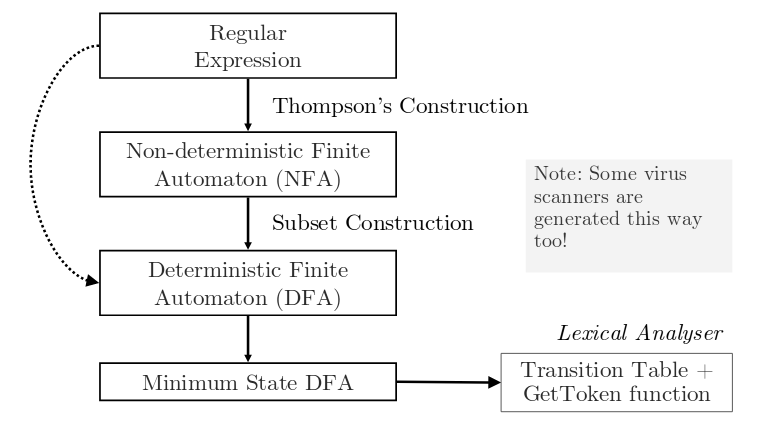
\includegraphics[width=0.75\linewidth]{img/lex}
\end{figure}


\subsection{Finite Automata}
\begin{itemize}
\item \emph{States} of matching process (circles).
\item \emph{Transitions} between those states (arrows).
\item Matched input \emph{symbols} (labels on transitions).
\item \emph{Accepting states} of matching process (double circle).
\item \emph{Start state} (unlabelled incoming arrow).
\end{itemize}

\paragraph{Deterministic Finite Automata}

No two transitions leaving a state have the same symbol.

\paragraph{Non-deterministic Finite Automata}

Allow a choice of transitions out of a state

\paragraph{Thompson's Construction}

Use $\epsilon$ transitions to glue together automata for each part
of a regex:

\begin{figure}[H]
\begin{centering}
\texttt{r1 r2}
\par\end{centering}
\centering{}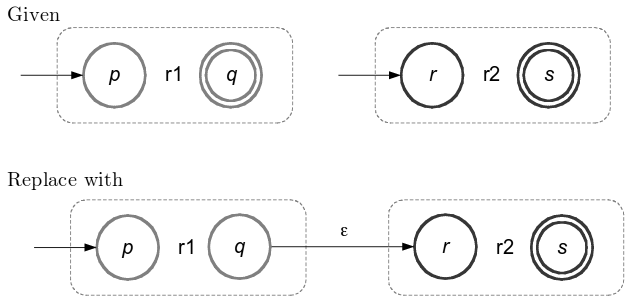
\includegraphics[width=0.5\linewidth]{img/concat}
\end{figure}

\begin{figure}[H]
\begin{centering}
\texttt{r1\textbar{}r2}
\par\end{centering}
\centering{}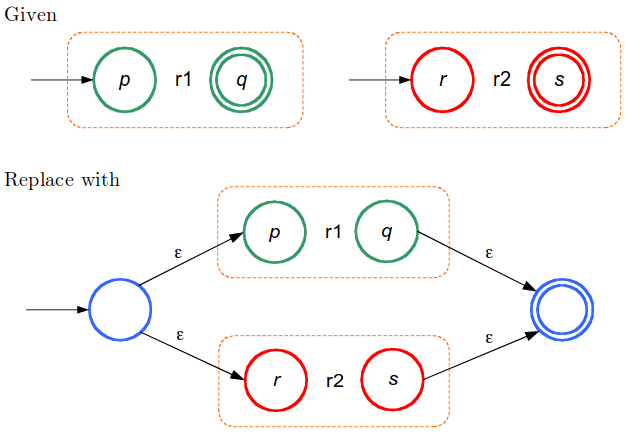
\includegraphics[width=0.5\linewidth]{img/alternate}
\end{figure}

\begin{figure}[H]
\begin{centering}
\texttt{r1{*}}
\par\end{centering}
\centering{}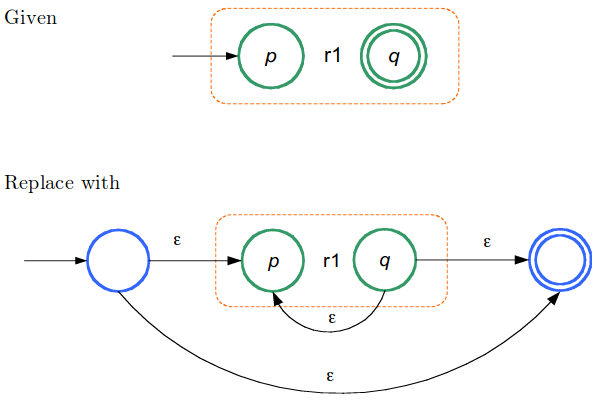
\includegraphics[width=0.5\linewidth]{img/repeat}
\end{figure}


\paragraph{Subset Construction}
\begin{itemize}
\item DFAs are much faster than NFAs (linear on size of input string), 
\item but require more memory (potentially $2^{n}$ states for an $n$-state
NFA).
\end{itemize}
\emph{Algorithm}:
\begin{enumerate}
\item DFA start state = $\epsilon$ closure of NFA start state.
\item For each new subset state $S$ of the DFA:
\begin{enumerate}
\item For each unique symbol \texttt{a} leading out from any state of $S$:
\begin{enumerate}
\item Add a transition \texttt{a} from S to S' where S' = $\epsilon$ closure
of states reached by \texttt{a}
\end{enumerate}
\end{enumerate}
\end{enumerate}

\paragraph{Generating a Lexical Analyser}

Encode DFA as a 2D table of states (row per state, col per char).
\end{document}
